%%
%% This is file `mcmthesis-demo.tex',
%% generated with the docstrip utility.
%%
%% The original source files were:
%%
%% mcmthesis.dtx  (with options: `demo')
%% 
%% -----------------------------------
%% 
%% This is a generated file.
%% 
%% Copyright (C)
%%     2010 -- 2015 by Zhaoli Wang
%%     2014 -- 2015 by Liam Huang
%% 
%% This work may be distributed and/or modified under the
%% conditions of the LaTeX Project Public License, either version 1.3
%% of this license or (at your option) any later version.
%% The latest version of this license is in
%%   http://www.latex-project.org/lppl.txt
%% and version 1.3 or later is part of all distributions of LaTeX
%% version 2005/12/01 or later.
%% 
%% This work has the LPPL maintenance status `maintained'.
%% 
%% The Current Maintainer of this work is Liam Huang.

%% 
\documentclass{mcmthesis}
\mcmsetup{tcn = 233666, problem = B,
sheet = true, titleinsheet = true, keywordsinsheet = true,
titlepage = true, abstract = true}
\usepackage{palatino}
\usepackage{mwe}
\usepackage{amsmath}
\usepackage{indentfirst}
\usepackage{graphicx}
\usepackage{subfigure}
\usepackage{caption}
\usepackage{framed}
\newcommand{\tabincell}[2]{\begin{tabular}{@{}#1@{}}#2\end{tabular}}  

\setlength{\itemsep}{0pt}
\setlength{\parindent} {2em}
\title{Sudoku Analyzing}
\author{Kai Feng, Song Lu, Yutao Zeng }
\date{\today}
\begin{document}
\begin{abstract}
here is the abstract!~!!
\begin{keywords}
keyword1; keyword2
\end{keywords}
\end{abstract}
\maketitle

\section{Introduction}
\subsection{Statement of Problem}
We set out to design an algorithm that would construct unique sudoku puzzles of various difficulties as well as to develop metrics by which to measure the difficulty of a given puzzle. In particular, our algorithm must admit at least four levels of difficulty while minimizing its level of complexity.

\subsection{Significance of Sudoku Research}
Sudoku is one of the most pupular puzzle games of all time, which is famous for its simple rules and puzzle diversity. We think that this problem is insteresting and of great significance, due to its inherently mathematical, and offers us an oppotunity to explore new mathematical techniques. After studying, we found out that this problem could be regarded as a derivation of the Latin Square puzzle, and can be solved by using the exact-cover method.\\
\indent Meanwhile, both solving and building the Sudoku puzzles are proved to be NP-Complete problems, which means that there is no known efficient way to locate an exact solution in the first place. It is apparently a great challenge for us to solve the problem in the polymonial time right now. But if we can make some progress,we may also expand into other and more practical problems. However, we shall restrict our focus directly to the problem at hand, and be content to leave these reasons, along with sudoku's entertainment value, as our motivation for exploring the game. 

\subsection{Sudoku Introduction}
Sudoku, is a logic-based,combinatorial number-placement puzzle. The objextive is to fill a $9\times9$ grid with digits so that each column, each row, and each of the nine $3\times3$ subgrids that compose the grid contains all of the digits from 1 to 9. The puzzle setter provides a partially completed grid, which for a well-posed puzzle has a unique solution. Figure.1(a) is a typical example of sudoku puzzle.

\begin{figure}[htbp]
\centering %居中
\subfigure[Typical sudoku puzzle]{ %第一张子图
\begin{minipage}{7cm}
\centering %子图居中
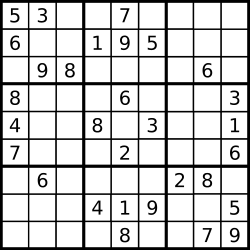
\includegraphics[scale=0.6]{figures/sudoku.png} %以pic.jpg的0.5倍大小输出
\end{minipage}
}
\subfigure[The same puzzle with solution]{ %第二张子图
\begin{minipage}{7cm}
\centering %子图居中
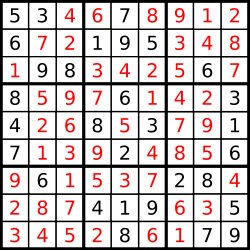
\includegraphics[scale=0.6]{figures/sudoku_complete.png} %以pic.jpg的0.5倍大小输出
\end{minipage}
}
\caption{sudoku puzzle instance} % %大图名称
\label{fig:1.3.1} %图片引用标记
\end{figure}

% \begin{figure}[htbp]
% \small
% \centering
% 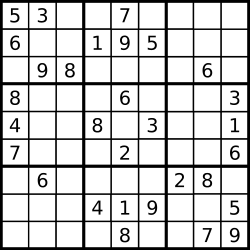
\includegraphics[width=6cm]{figures/sudoku.png}
% \caption{Typical sudoku puzzle} \label{fig:1.1}
% \end{figure}

\indent Completed games are always a type of Latin square with an additional constraint on the contents of individual regions. For example, the same single integer may not appear twice in the same row, column, or any of the nine $3\times3$ subregions of the $9\times9$ playing board.\newline

% \centerline{
% 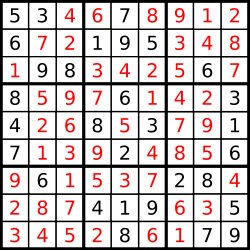
\includegraphics[width = 6cm]{figures/sudoku_complete.png}
% }
% \centerline{Fig.2 }

\subsection{Notations and Terminologies}
It is difficult to discuss our solution to the proposed problem without understanding some common
terminology. Moreover, since we will apply more mathematical formalism here than in most documents dealing with sudoku, it will be helpful to introduce notational conventions.

\begin{itemize}
	\item \textbf{Cell.} The basic unit of Sudoku puzzle. A square in the grid which may contain one digit(1-9). The grid is composed of 81 cells.

	\item \textbf{Block.} A $3\times3$ array of cells. Normally, the boundaries of the blocks are marked by slightly darker or thicker lines than the lines separating the cells. The grid is composed of 9 non-overlapping blocks. Each block must contain all the digits(form 1 to 9) and may not contain more than one of each digit.

	\item \textbf{Column.} A verticle line of 9 cells. The grid is composed of 9 columns. Each column must contain all the digits(1-9) and may not contain more than one of each digit.

	\item \textbf{Row.} A horizontal line of 9 cells. The grid is composed of 9 rows. Each row must contain all the digits (1-9) and may not contain more than one of each digit.

	\item \textbf{Grid.} The $9\times9$ array of cells that compose a Sudoku puzzle. The grid contains 9 rows, 9 columns and 9 blocks.

	\item \textbf{Puzzle.} A $9\times9$ matrix of cells, with at least one empty and at least one filled cell. For our purposes, we impose the additional requirement that all puzzles have exactly one solution. 	

	\item \textbf{House.} The column, row and block are collectively called the House.

	\item \textbf{Peer.} If two cells are in the same house (same row, same column, or same block) they are said to see each other, or to be peers.


	\item \textbf{Candidate.} Any digit that may be placed in an empty cell based on current state of the puzzle. If a digit is present in one or more of a cell's buddies, it cannot be a candidate for that cell. Analysis may further reduce the candidate set to a signle candidate, that candidate must be the sulution for that cell.

	\item \textbf{Analysis.} Any technique that eliminates candidates. Techniques of analysis do ultimately lead to solutions for cells, but it may take the application of multiple techniques or multiple applications of the same technique to reach a solution for a single cell. The point of analysis then, is to eliminate candidates, not look for solutions. Looking for solutions is scanning.
\end{itemize}

\subsection{Common Solving Strategy}
\subsubsection{Full House/Last Digit}
A Full House is simply the last digit that can be placed in a row,column or block. If it is the last digit for the whole grid, it is sometimes called "Last Digit".

\begin{figure}[ht]
\small
\centering
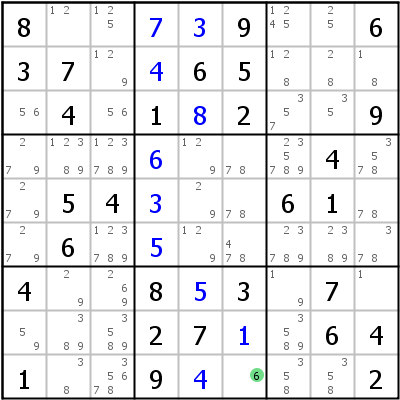
\includegraphics[width=7cm]{figures/full_house.png}
\caption{an example of full house} \label{fig:1.5.1}
\end{figure}

\subsubsection{Naked Single}
Naked Single means that in a specific cell only one digit remains possible (the last remaining candidate has no other candidates to hide behind and is thus naked). The digit must then go into that cell.

\begin{figure}[htbp]
\centering %居中
\subfigure[Naked Single]{ %第一张子图
\begin{minipage}{7cm}
\centering %子图居中
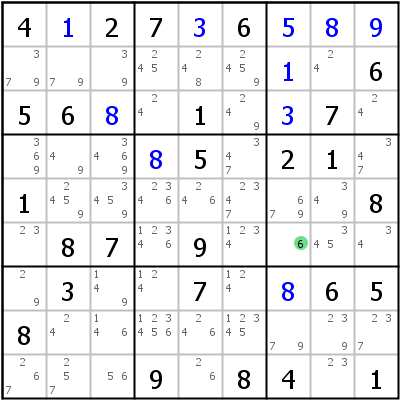
\includegraphics[scale=0.65]{figures/naked_single.png} %以pic.jpg的0.5倍大小输出
\end{minipage}
}
\subfigure[Hidden Single]{ %第二张子图
\begin{minipage}{7cm}
\centering %子图居中
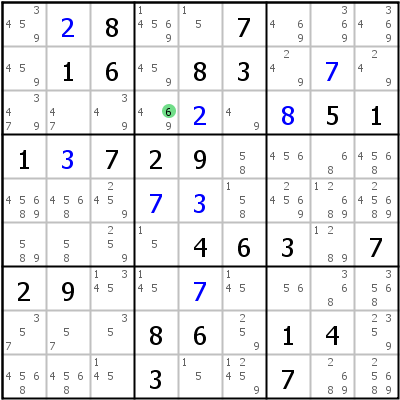
\includegraphics[scale=0.65]{figures/hidden_single.png} %以pic.jpg的0.5倍大小输出
\end{minipage}
}
\caption{Single Strategy} % %大图名称
\label{fig:1.5.2} %图片引用标记
\end{figure}

\subsubsection{Hidden Single}
Hidden Single means that for a given digit and house only one cell is left to place that digit. The cell itself has more than one candidate left, the correct digit is thus hidden amongst the rest.

\subsubsection{Naked Pair}
If you can find two cells, both in the same house, that have only the same two candidates left, you can eliminate that two candidates from all other cells in that house.

\subsubsection{Hidden Pair}
All Hidden Subsets work the same way, the only thing that changes is the number of cells and candidates affected by the move. Take Hidden Pair: If you can find two cells within a house such as that two candidates appear nowhere outside those cells in that house, those two candidates must be placed in the two cells. All other candidates can therefore be eliminated.

\begin{figure}[htbp]
\centering
\subfigure[Naked Pair]{
	\begin{minipage}{7cm}
	\centering
	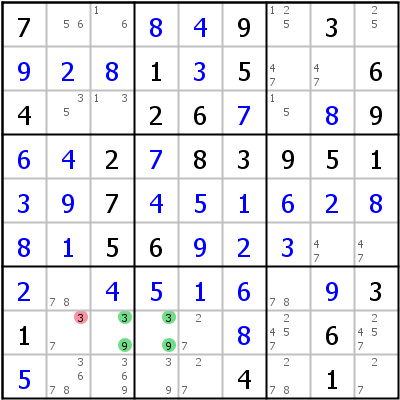
\includegraphics[scale = 0.65]{figures/naked_paire.png}
	\end{minipage}
}
\subfigure[Hidden Pair]{
	\begin{minipage}{7cm}
	\centering
	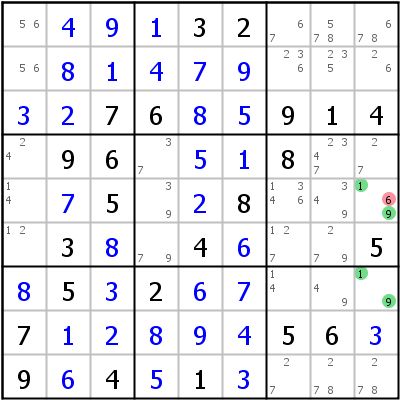
\includegraphics[scale = 0.65]{figures/hidden_pair.png}
	\end{minipage}
}
\caption{Pair Strategy}
\label{fig:1.5.3}
\end{figure}



\subsubsection{Hidden Triple}
Hidden Triples work in the same way as Hidden Pairs only with three cells and three candidates.\newline

All the strategies above will be used as the benchmark to test the difficulty of new-created sudoku puzzles.

\section{Analysis of the Problem}
\subsection{Background Knowledge}

\subsubsection{Exact Cover}
In mathematics, given a collection $\mathcal{S}$ of subsets of a set $\mathcal{X}$, an \textbf{exact vocer} is a subcollection $\mathcal{S^*}$ of $\mathcal{S}$ that satisfies two conditions:
\begin{itemize}
	\item The intersection of any two sistinct subsets in $\mathcal{S^*}$ is empty, i.e., the subsets in $\mathcal{S^*}$ are pairwise disjoint. In other words, each element in $\mathcal{X}$ is contained in at most one subset in $\mathcal{S^*}$.
	\item The union of the subsets in $\mathcal{S^*}$ is $\mathcal{X}$, i.e., the subsets in $\mathcal{S^*}$ cover $\mathcal{X}$. In other words, each element in $\mathcal{X}$ is contained in at least one subset in $\mathcal{S^*}$.
\end{itemize}

\indent In short, an exact cover is "exact" in the sense that each element in $\mathcal{X}$ is contained in exactly one subset in $\mathcal{S^*}$. Figure 5 is an example of exact cover. As we can see the set(row 1,4 and 5) is the exact cover of the origin matrix.

\begin{figure}[htbp]
\small
\centering
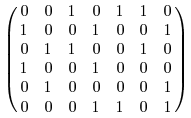
\includegraphics[width=4cm]{figures/exact_cover.png}
\caption{an example of exact cover} \label{fig:2.1.1}
\end{figure}

\subsubsection{Algorithm X}
To solve the exact cover problem, we need to introduce the methodology called Algorithm X. "Algorithm X" is the name D.E Knuth used in his paper "Dancing Links" to refer to "the most obvious-trail-and-error approach" for finding all solutions to the exact cover problem. Technically, Algorithm X is a recursive, nondeterministic, depth-first, backtracking algorithm. While Algorithm X is generally useful as a succinct explanation of how the exact cover problem may be solved, Knuth's intent in presenting it was merely to demonstrate the utility of the dancing links technique via an efficient implementation he called DLX.\newline
\indent The exact cover problem is represented in Algorithm X using a matrix A consisting of 0s and 1s. The goal is to select a subset of the rows so that the digit 1 appears in each column exactly once. Algorithm X functions as follows:\\
\begin{framed}
\newcounter{alg}
\begin{list}{\arabic{alg}.}
    {\usecounter{alg}\setlength{\parsep}{0ex}\setlength{\itemsep}{0ex}}
\item[] Algorithm X
\item   If the matrix \textit{A} has no columns, the current partial solution is a valid solution; terminate successfully.
\item   Otherwise choose a column \textit{c} (deterministically).
\item 	Choose a row \textit{r} such that $A_{r, c} = 1$ (nondeterministically).
\item For each column \textit{j} such that $A_{r, j} = 1$, 
\item[] \qquad for each row \textit{i} such that $A_{i,j} = 1$,
\item[] \qquad \qquad delete row \textit{i} from matrix \textit{A},
\item[] \qquad delete column \textit{j} from matrix \textit{A}.
\item Repeat this algorithm recursively on the reduced matrix \textit{A}.
\end{list}
\end{framed}

For better understanding the procedure of Algorithm X, let's see the following example. Consider the exact problem specified by the universe U = \{1, 2, 3, 4, 5, 6, 7\} and the collection of sets $\mathcal{S}$ = \{\textit{A, B, C, D, E, F}\}, where:
\begin{itemize}
	\item \textit{A} = \{1, 4, 7\};
	\item \textit{B} = \{1, 4\};
	\item \textit{C} = \{4, 5, 7\};
	\item \textit{D} = \{3, 5, 6\};
	\item \textit{E} = \{2, 3, 6, 7\};
	\item \textit{F} = \{2, 7\};
\end{itemize}

This problem is presented by the matrix:
\begin{table}[ht]
\centering
	\begin{tabular}{|r|r|r|r|r|r|r|r|}
		\hline
		     & 1 & 2 & 3 & 4 & 5 & 6 & 7\\
		     \hline
		   A & 1 & 0 & 0 & 1 & 0 & 0 & 1\\
		     \hline
		   B & 1 & 0 & 0 & 1 & 0 & 0 & 0\\
		     \hline
		   C & 0 & 0 & 0 & 1 & 1 & 0 & 1\\
		     \hline
		   D & 0 & 0 & 1 & 0 & 1 & 1 & 0\\
		     \hline
		   E & 0 & 1 & 1 & 0 & 0 & 1 & 1\\
		     \hline
		   F & 0 & 1 & 0 & 0 & 0 & 0 & 1\\
		\hline
	\end{tabular}
\caption{Origin Matrix}
\end{table}

For the least recursive time, we often select the column with the least 1s to start. Let's go on and solve this problem. 

\textbf{Level 0}\\
\indent Step 1 -- The matrix is not empty, so the algorithm proceeds. \\
\indent Step 2 -- The lowest number of 1s in any column is two. Column 1 is the first column with two 1s and thus is selected(deterministically):

\begin{table}[ht]
\centering
	\begin{tabular}{|r|r|r|r|r|r|r|r|}
		\hline
		     & 1 & 2 & 3 & 4 & 5 & 6 & 7\\
		     \hline
		   A & \textcolor[rgb]{0.98,0.00,0.00}1 & 0 & 0 & 1 & 0 & 0 & 1\\
		     \hline
		   B & \textcolor[rgb]{0.98,0.00,0.00}1 & 0 & 0 & 1 & 0 & 0 & 0\\
		     \hline
		   C & 0 & 0 & 0 & 1 & 1 & 0 & 1\\
		     \hline
		   D & 0 & 0 & 1 & 0 & 1 & 1 & 0\\
		     \hline
		   E & 0 & 1 & 1 & 0 & 0 & 1 & 1\\
		     \hline
		   F & 0 & 1 & 0 & 0 & 0 & 0 & 1\\
		\hline
	\end{tabular}
\end{table}

\indent Step 3 -- Rows \textit{A} and \textit{B} each have a 1 in column 1 and thus are selected (nondeterministically).\\
The algorithm moves to the first branch at level 1.

\textbf{Level 1: Select Row A} \\
\indent Step 4 -- Row \textit{A} is included in the partial solution.\\
\indent Step 5 -- Row \textit{A} has a 1 in columns 1, 4, and 7:

\begin{table}[ht]
\centering
	\begin{tabular}{|r|r|r|r|r|r|r|r|}
		\hline
		     & \textcolor[rgb]{0.00,0.00,0.98}1 & 2 & 3 & \textcolor[rgb]{0.00,0.00,0.98}4 & 5 & 6 & \textcolor[rgb]{0.00,0.00,0.98}7\\
		     \hline
		   \textcolor[rgb]{0.98,0.00,0.00}A & \textcolor[rgb]{0.98,0.00,0.00}1 & 0 & 0 & \textcolor[rgb]{0.98,0.00,0.00}1 & 0 & 0 & \textcolor[rgb]{0.98,0.00,0.00}1\\
		     \hline
		   B & 1 & 0 & 0 & 1 & 0 & 0 & 0\\
		     \hline
		   C & 0 & 0 & 0 & 1 & 1 & 0 & 1\\
		     \hline
		   D & 0 & 0 & 1 & 0 & 1 & 1 & 0\\
		     \hline
		   E & 0 & 1 & 1 & 0 & 0 & 1 & 1\\
		     \hline
		   F & 0 & 1 & 0 & 0 & 0 & 0 & 1\\
		\hline
	\end{tabular}
\end{table}

\indent Column 1 has a 1 in rows \textit{A} and \textit{B}; column 4 has a 1 in rows \textit{A}, \textit{B}, and \textit{C}; and column 7 has a 1 in rows \textit{A}, \textit{C}, \textit{E}, and \textit{F}. Thus rows \textit{A}, \textit{B}, \textit{C}, \textit{E}, and \textit{F} are to be removed and columns 1, 4 and 7 are to be removed:

\begin{table}[ht]
\centering
	\begin{tabular}{|r|r|r|r|r|r|r|r|}
		\hline
		     & \textcolor[rgb]{0.98,0.00,0.00}1 & 2 & 3 & \textcolor[rgb]{0.98,0.00,0.00}4 & 5 & 6 & \textcolor[rgb]{0.98,0.00,0.00}7\\
		     \hline
		   \textcolor[rgb]{0.00,0.00,0.98}A & \textcolor[rgb]{0.98,0.00,0.00}1 & 0 & 0 & \textcolor[rgb]{0.98,0.00,0.00}1 & 0 & 0 & \textcolor[rgb]{0.98,0.00,0.00}1\\
		     \hline
		   \textcolor[rgb]{0.00,0.00,0.98}B & \textcolor[rgb]{0.98,0.00,0.00}1 & 0 & 0 & \textcolor[rgb]{0.98,0.00,0.00}1 & 0 & 0 & 0\\
		     \hline
		   \textcolor[rgb]{0.00,0.00,0.98}C & 0 & 0 & 0 & \textcolor[rgb]{0.98,0.00,0.00}1 & 1 & 0 & \textcolor[rgb]{0.98,0.00,0.00}1\\
		     \hline
		   D & 0 & 0 & 1 & 0 & 1 & 1 & 0\\
		     \hline
		   \textcolor[rgb]{0.00,0.00,0.98}E & 0 & 1 & 1 & 0 & 0 & 1 & \textcolor[rgb]{0.98,0.00,0.00}1\\
		     \hline
		   \textcolor[rgb]{0.00,0.00,0.98}F & 0 & 1 & 0 & 0 & 0 & 0 & \textcolor[rgb]{0.98,0.00,0.00}1\\
		\hline
	\end{tabular}
\end{table}

Row D remains and columns 2, 3, 5, and 6 remain:\\

\begin{table}[ht]
\centering
	\begin{tabular}{|r|r|r|r|r|}
	\hline
	  & 2 & 3 & 5 & 6\\
	\hline
	D & 0 & 1 & 1 & 1\\
	\hline
	\end{tabular}
\end{table}

Step 1 -- The matrix is not empty, so the algorithm proceeds.\\
\indent Step 2 -- The lowest number of 1s in any column is zero and column 2 is the first column with zero 1s:\\
\begin{table}[!ht]
\centering
	\begin{tabular}{|r|r|r|r|r|}
	\hline
	  & \textcolor[rgb]{0.98,0.00,0.00}2 & 3 & 5 & 6\\
	\hline
	D & 0 & 1 & 1 & 1\\
	\hline
	\end{tabular}
\end{table}

Thus this branch of the algorithm terminates unsuccessfully. The algorithm moves to the next branch at level 1.

\textbf{Level 1: Select Row B}\\
\indent Step 4 -- Row \textit{B} is included in the partial solution.Row \textit{B} has a 1 in columns 1 and 4:\\
\begin{table}[ht]
\centering
	\begin{tabular}{|r|r|r|r|r|r|r|r|}
		\hline
		     & \textcolor[rgb]{0.00,0.00,0.98}1 & 2 & 3 & \textcolor[rgb]{0.00,0.00,0.98}4 & 5 & 6 & 7\\
		     \hline
		   A & 1 & 0 & 0 & 1 & 0 & 0 & 1\\
		     \hline
		   \textcolor[rgb]{0.98,0.00,0.00}B & \textcolor[rgb]{0.98,0.00,0.00}1 & 0 & 0 & \textcolor[rgb]{0.98,0.00,0.00}1 & 0 & 0 & 0\\
		     \hline
		   C & 0 & 0 & 0 & 1 & 1 & 0 & 1\\
		     \hline
		   D & 0 & 0 & 1 & 0 & 1 & 1 & 0\\
		     \hline
		   E & 0 & 1 & 1 & 0 & 0 & 1 & 1\\
		     \hline
		   F & 0 & 1 & 0 & 0 & 0 & 0 & 1\\
		\hline
	\end{tabular}
\end{table}

After several steps, we can get the matrix:\\

\begin{table}[!ht]
\centering
	\begin{tabular}{|r|r|r|}
	\hline
	 & 2 & 7 \\
	 \hline
	 F & 1 & 1 \\
	 \hline
	 \end{tabular}
\end{table}

Notice that the next step we can clear all the rest 1s in the matrix. So it is a correct answer to this exact cover problem. As rows \textit{B}, \textit{D}, and \textit{F} are selected, the final solution is:
\begin{table}[!ht]
\centering
	\begin{tabular}{|c|c|c|c|c|c|c|c|}
	\hline
	  & 1 & 2 & 3 & 4 & 5 & 6 & 7 \\
	  \hline
	B & 1 & 0 & 0 & 1 & 0 & 0 & 0 \\
	\hline
	D & 0 & 0 & 1 & 0 & 1 & 1 & 0 \\
	\hline
	F & 0 & 1 & 0 & 0 & 0 & 0 & 1 \\
	\hline
	\end{tabular}
\end{table}

% \subsubsection{Sudoku to Exact Cover}


\subsection{Model Building}
Now we have known how to solve the exact cover problem with Algorithm X, so what's the relationship between Sudoku puzzle and exact cover problem? In fact, generating and solving Sudoku are both exact cover problems. But apparently, Algorithm X are used to solve the 0-1 problem which is much different from the Sudoku grid. So the next thing we need to do is to convert Sudoku problem into the exact cover problem. Let me introduce some indices we might use later.\\

\begin{table}[!ht]
\centering
	\begin{tabular}{cc}
	\hline
	Symbols & Meanings \\
	\hline
	$\mathcal{X}$ & The set of candidates \\	
	$\mathcal{Y}$ & The set of constrains sets \\
	$\mathcal{R}$ & \tabincell{c}{Binary relation matrix with 324 columns and 729 rows \\
								 at most,representing the relationship "is contained in".}\\
	$\textit{c}_{i,j}$ & The element in R matrix, located in row i and column j. \\
	\hline
	\end{tabular}
\caption{Symbol Table}
\end{table}

Intuitively, we need to find a transformation \textit{T}, which could achieve: \newline

\centerline{$\textit{T}_{\mathcal{Y}}(X) = R$}
Each possible assignment of a particular number to a particular cell is a candidate. When Sudoku is played with pencil and paper, candidates are often called penceil marks. In the standard $9\times9$ Sudoku variant, in which each of $9\times9$ cells is assigned one of 9 numbers, there are $9\times9\times9=729$ possibilities. The key to convert Sudoku into exact cover problem is to find out the constrains sets $\mathcal{Y}$. According to the rules of Sudoku, we can get following constains: \newline
\begin{itemize}
	\item Each cell \textbf{must} and \textbf{only} have one digit.
	\item No duplicate number in the same row.
	\item No duplicate number in the same column.
	\item No duplicate number in the same block.
\end{itemize}

\indent All the constaints are listed above, let's build the matrix R step by step. As we all Sudoku grid has 81 cells and a completed Sudoku has one digit in each of its cell. So in order to represent this constraint, we need 81 rows in our matrix $\mathcal{R}$. The elements in each row are not digit(1-9), but a abstract bool value(0 or 1). 1 means this cell has a number, otherwise it should be 0. Here we assign the number to the cell from left to right, starting from the top row. So if $\textit{c}_{i,j}$ is not null, the $(9\times i + j)th$ row should be 1. We call these 81 lines combined as "cell field" Apparently, a correct solution of Sudoku should be the exact cover of cell field.\\
\indent We need no duplicate numbers in the same row, which means each number can only be placed once in a single row. There are 9 digits and 9 rows in a grid, so we also need 81 rows to express this constraint, called "row field". The column 1 to column 9 of the row field shows that the Sudoku has digit 1 to 9 in the first row, column 10 to 18 are correspond to the second row and so on. If we have placed digit 8 in the seventh row, then the $6\times9+8=62nd$ column should be marked as 1. A corrent solution could also be the exact cover of row field.\\
\indent Just like "row field", "column field" are quite the same,which represents whether one digit has shown up in one column.If you have digit 8 in the 7th column, then the  $6\times9+8=62nd$ column should be marked as 1.\\
\indent Let's come to the last constraints. There are 9 digits and 9 blocks in a Sudoku, which means we need another 81 columns to express the relationship, called "block field". The index are count from the left-top to the right-bottom, rows first. \\
\indent Now we can join all the four fields above and get the matrix with 324 columns. A Sudoku problem should have atmost 729 rows(for all possibilities). This matrix is the matrix $\mathcal{R}$ and the job to solve the Sudoku puzzle now has changed to find a exact cover of this matrix. \newline 
\section{Matrix Design}
\indent To generate Sudoku puzzles of varying difficulty in a effcient way, we decide to split it into two parts.The first part is to generate a complete Sudoku grid filled with $9\times9$ figures. And the second part is to dig a few figures from the complete Sudoku grid. Of course, we need to gurantee that the Sudoku has a unique solution.\\
\subsection{Generate complete Sudoku grids}
\indent There is a fact that the number of different complete Sudoku grids was computed to be $6670903752021072936960 \approx 6.671 \times 10^{21}$. And the essentially different Sudoku grids, which can not be transformed by another Sudoku grid in some symmetrical ways, is proved to be $2297902829591040$ by Ed Russell and Frazer Jarvis in 2006. That's to say, the possiblity of building a random Sudoku grid is high enough for computers. Based on this, we adopt a Las Vegas-liked algorithm to generate them.\\
\indent First of all, we create a random array filled with $1\sim9$ and put it in the first line of a empty Sudoku grid. Then we continue to create a array, take the figures out of it in turns to fill in cells of the follwing line, and check  whether the constraints are met. If not, we put the figures back and check next figure until the line is completely filled. If this process fails, a new random array is needed to be created. Then repeat the procedure. \\
\indent Here is the pseudocode:\\
\begin{framed}
\newcounter{GenerateSudoku}
\begin{list}{\arabic{GenerateSudoku}.}
    {\usecounter{GenerateSudoku}\setlength{\parsep}{0ex}\setlength{\itemsep}{0ex}}
\item[] Generate Complete Grids Algorithm
\item Define a array \textit{A} which is filled with $1\sim9$ in turns. 
\item Choose a random figure in this array and swap it with A[0]. Repeat the procedure for a few (in most cases, the number is 20) times. Then the array \textit{A} becomes a random one.
\item For each line \textit{i} in a empty Sudoku \textit{S},
\item[] \qquad if it's the first line($\textit{i} = 0$),
\item[] \qquad \qquad put the array in without any check,
\item[] \qquad else if $\textit{i} \ne 0$,
\item[] \qquad \qquad randomize the array \textit{A} with Step 2,
\item[] \qquad \qquad for each figure \textit{n} in \textit{A},
\item[] \qquad \qquad \qquad fill the cells in $S_i$ with \textit{n} that can be put in, 
\item[] \qquad \qquad if $S_i$ can't be filled up,
\item[] \qquad \qquad \qquad randomize array \textit{A},
\item[] \qquad \qquad \qquad if the randomization times \textit{t} reach a threshold \textit{MaxTimes},
\item[] \qquad \qquad \qquad \qquad remove all figures in \textit{S} and restart( procedure for \textit{i} in \textit{S} )
\item[] \qquad \qquad \qquad else,
\item[] \qquad \qquad \qquad \qquad remove all the figures in $S_i$ and repeat procedure($\textit{i} \ne 0$) ,
\item return the complete Sudoku \textit{S}.
\end{list}
\end{framed}
\indent Obviously, by trying for enough times, we will get a complete Sudoku grid which meets all the constraints. In fact, we can generate such grids in several milliseconds, in other words, $100000$ grids in one minute. By the way, digging different figures in different orders from a complete Sudoku grid will generate a large amount of Sudoku puzzles. Therefore, this Las Vegas-liked algorithm is quite efficient and our require to construct various Sudoku puzzles can be met quite well.\\

\section{The Model Results}


\section{Evaluate of the Model}
\subsection{Advantage of the Model}
\subsection{Disadvantage of the Model}

\section{Validating the Model}


\section{Conclusions}
in short but accurate

\section{A Summary}
\lipsum[6]
lipsum latex

\section{Strengths and weaknesses}
\lipsum[12]

\subsection{Strengths}
\begin{itemize}
	\item \textbf{Applies widely}\\
	This  system can be used for many types of airplanes, and it also
	solves the interference during  the procedure of the boarding
	airplane,as described above we can get to the  optimization
	boarding time.We also know that all the service is automate.
	\item \textbf{Improve the quality of the airport service}\\
	Balancing the cost of the cost and the benefit, it will bring in
	more convenient  for airport and passengers.It also saves many
	human resources for the airline. \item \textbf{}
\end{itemize}

\begin{thebibliography}{99}
\bibitem{1} Donald E. Knuth: Dancing Links, Oxford-Microsoft Symposium on Computer Science, 2000
\bibitem{2}	Wikipedia: Sudoku
\bibitem{3}\url{http://blog.gssxgss.me/use-dlx-to-solve-sudoku-1/}
\end{thebibliography}

\begin{appendices}

\section{First appendix}

Here are simulation programmes we used in our model as follow.\\

% \textbf{\textcolor[rgb]{0.98,0.00,0.00}{Input java source:}}
\centering
Listing 1 : Implement of Sudoku Creation
\lstinputlisting[language=Java]{./code/src/Sudoku/Array.java}
\lstinputlisting[language=Java]{./code/src/Sudoku/ColumnHead.java}
\lstinputlisting[language=Java]{./code/src/Sudoku/GenerateByLasVegas.java}
\lstinputlisting[language=Java]{./code/src/Sudoku/GenerateFullSudoku.java}
\lstinputlisting[language=Java]{./code/src/Sudoku/GetPuzzle.java}
\lstinputlisting[language=Java]{./code/src/Sudoku/Main.java}
\lstinputlisting[language=Java]{./code/src/Sudoku/Resolve.java}
\lstinputlisting[language=Java]{./code/src/Sudoku/Sudoku.java}
\lstinputlisting[language=Java]{./code/src/Sudoku/SudokuNode.java}
\lstinputlisting[language=Java]{./code/src/Sudoku/TranslateSolution.java}

\section{Second appendix}
some more text \textcolor[rgb]{0.98,0.00,0.00}{\textbf{Input C++ source:}}
\lstinputlisting[language=C++]{./code/mcmthesis-sudoku.cpp}

\end{appendices}
\end{document}

%% 
%% This work consists of these files mcmthesis.dtx,
%%                                   figures/ and
%%                                   code/,
%% and the derived files             mcmthesis.cls,
%%                                   mcmthesis-demo.tex,
%%                                   README,
%%                                   LICENSE,
%%                                   mcmthesis.pdf and
%%                                   mcmthesis-demo.pdf.
%%
%% End of file `mcmthesis-demo.tex'.
